\documentclass[12pt,a4paper]{article}

\usepackage[utf8]{inputenc}
\usepackage[T1]{fontenc}
\usepackage[spanish, es-nodecimaldot]{babel}
\usepackage{geometry}
\usepackage{graphicx}
\usepackage{float}
\usepackage{booktabs}
\usepackage{array}
\usepackage{xcolor}
\usepackage{amsmath}
\usepackage{listings}
\usepackage{hyperref}
\usepackage{fancyhdr}
\usepackage{titlesec}

\geometry{
left=1in,
right=1in,
top=1in,
bottom=1in
}

\pagestyle{fancy}
\fancyhf{}
\lhead{Práctica 2: OSPF}
\rhead{Interacción de redes}
\cfoot{\thepage}

% Configuración de código
\definecolor{codegray}{gray}{0.95}

\lstdefinestyle{cisco}{
backgroundcolor=\color{codegray},
basicstyle=\ttfamily\small,
frame=single,
breaklines=true,
columns=fullflexible,
keepspaces=true,
showstringspaces=false
}

\hypersetup{
colorlinks=true,
linkcolor=black,
urlcolor=blue,
citecolor=black
}

\title{
Práctica 3: OSPF - DHCP\\[0.5em]
\large Interacción de redes
}

\author{
Jorge Alberto Suarez Saldana\\
\small Matrícula: 355992\\
\small Profesor: Raymundo Antonio González Grimaldo
}

\date{\today}

\begin{document}

\maketitle

\section{Introducción}

En esta práctica se realizó la configuración de una topología de red compuesta por varios routers, switches, equipos finales y un router ISP. El objetivo principal fue implementar un esquema de enrutamiento dinámico mediante OSPF, configurar la asignación automática de direcciones IPv4 mediante DHCP y comprobar la conectividad entre las diferentes redes de la topología.

Además de la configuración inicial, la práctica permitió analizar problemas reales de conectividad ocasionados por errores en la conexión física de las interfaces seriales, configuraciones antiguas que permanecían en los routers y la ausencia de rutas de retorno desde el router ISP hacia las redes internas.

El proceso de solución permitió relacionar directamente la configuración de las interfaces, las tablas de enrutamiento, las vecindades OSPF, las rutas por defecto y el funcionamiento de DHCP.

\section{Objetivos}

\begin{itemize}
\item Configurar las interfaces de los routers utilizando el direccionamiento IPv4 correspondiente a la topología.
\item Establecer conectividad entre los routers mediante enlaces seriales.
\item Configurar OSPF como protocolo de enrutamiento dinámico.
\item Establecer las vecindades OSPF entre los routers de la red interna.
\item Configurar R4 como servidor DHCP para las redes LAN conectadas a S3 y S4.
\item Verificar la asignación automática de direcciones IP en los equipos finales.
\item Configurar una ruta por defecto desde R1 hacia el router ISP.
\item Propagar la ruta por defecto mediante OSPF hacia los demás routers.
\item Configurar las rutas necesarias en el ISP para permitir el tráfico de regreso hacia las redes internas.
\item Comprobar la conectividad extremo a extremo mediante pruebas de ping.
\end{itemize}

\section{Topología}

La topología utilizada durante la práctica se muestra en la Figura~\ref{fig:topologia}.

\begin{figure}[H]
\centering

\includegraphics[width=\textwidth]{topologia.png}
\caption{Topología de red utilizada en la práctica.}
\label{fig:topologia}
\end{figure}

La red está compuesta por los routers R1, R2, R3, R4 e ISP. R1 funciona como punto de conexión entre la red interna y el ISP. Los routers R1, R2, R3 y R4 utilizan OSPF para intercambiar información de enrutamiento.

R4 proporciona conectividad a las redes LAN de S3 y S4 y funciona además como servidor DHCP para ambas redes.

El router ISP posee una red directamente conectada hacia R1 y otra red LAN donde se encuentra el servidor utilizado para comprobar la conectividad externa.

\section{Esquema de direccionamiento}

El direccionamiento utilizado para los principales enlaces y redes LAN se muestra en la Tabla~\ref{tab:direccionamiento}.

\begin{table}[H]
\centering
\caption{Direccionamiento IPv4 de la topología.}
\label{tab:direccionamiento}
\small

\begin{tabular}{llll}
\toprule
Dispositivo & Interfaz & Dirección IP & Red \\
\midrule
R1 & S0/3/0 & 140.10.0.1/24 & 140.10.0.0/24 \\
R1 & S0/3/1 & 52.0.0.1/24 & 52.0.0.0/24 \\
R1 & G0/0 & 206.10.5.1/24 & 206.10.5.0/24 \\
\midrule
R2 & S0/3/1 & 140.10.0.2/24 & 140.10.0.0/24 \\
R2 & S0/3/0 & 140.30.0.1/24 & 140.30.0.0/24 \\
R2 & S0/2/1 & 140.0.0.1/24 & 140.0.0.0/24 \\
R2 & G0/0 & 205.20.3.1/24 & 205.20.3.0/24 \\
\midrule
R3 & S0/3/1 & 140.30.0.2/24 & 140.30.0.0/24 \\
R3 & S0/3/0 & 140.20.0.1/24 & 140.20.0.0/24 \\
\midrule
R4 & S0/3/0 & 140.0.0.2/24 & 140.0.0.0/24 \\
R4 & S0/3/1 & 140.20.0.2/24 & 140.20.0.0/24 \\
R4 & G0/0 & 148.10.144.1/24 & 148.10.144.0/24 \\
R4 & G0/1 & 148.10.176.1/24 & 148.10.176.0/24 \\
\midrule
ISP & S0/3/0 & 52.0.0.2/24 & 52.0.0.0/24 \\
ISP & G0/0 & 52.0.1.1/24 & 52.0.1.0/24 \\
\bottomrule
\end{tabular}
\end{table}

Los equipos conectados a S1 y S2 utilizan direcciones estáticas. Las redes de S3 y S4 utilizan DHCP.

\section{Configuración de OSPF}

Se utilizó el proceso OSPF número 10 y el área 0. Para facilitar la identificación de cada router se establecieron los siguientes Router ID:

\begin{table}[H]
\centering
\caption{Identificadores de los routers OSPF.}
\begin{tabular}{ll}
\toprule
Router & Router ID \\
\midrule
R1 & 1.1.1.1 \\
R2 & 2.2.2.2 \\
R3 & 3.3.3.3 \\
R4 & 4.4.4.4 \\
\bottomrule
\end{tabular}
\end{table}

Las redes internas fueron anunciadas mediante declaraciones \texttt{network} con máscaras wildcard correspondientes a redes /24.

Por ejemplo, la configuración de OSPF en R1 incluye:

\begin{lstlisting}[style=cisco]
router ospf 10
router-id 1.1.1.1
network 140.10.0.0 0.0.0.255 area 0
network 52.0.0.0 0.0.0.255 area 0
network 206.10.5.0 0.0.0.255 area 0
\end{lstlisting}

El uso de OSPF permite que los routers R1, R2, R3 y R4 aprendan dinámicamente las diferentes redes de la topología sin tener que configurar manualmente rutas estáticas entre todos ellos.

\subsection{Verificación de R1}

La siguiente sección está destinada a colocar la salida del comando \texttt{show ip protocols} ejecutado en R1.

\begin{verbatim}
R1>show ip protocols

Routing Protocol is "ospf 10"
  Outgoing update filter list for all interfaces is not set 
  Incoming update filter list for all interfaces is not set 
  Router ID 1.1.1.1
  It is an autonomous system boundary router
  Redistributing External Routes from,
  Number of areas in this router is 1. 1 normal 0 stub 0 nssa
  Maximum path: 4
  Routing for Networks:
    140.10.0.0 0.0.0.255 area 0
    52.0.0.0 0.0.0.255 area 0
    206.10.5.0 0.0.0.255 area 0
  Routing Information Sources:  
    Gateway         Distance      Last Update 
    1.1.1.1              110      00:15:51
    2.2.2.2              110      00:15:52
    3.3.3.3              110      00:15:52
    4.4.4.4              110      00:15:51
  Distance: (default is 110)

R1>
\end{verbatim}

A continuación se coloca la salida de la tabla de enrutamiento de R1.

\begin{verbatim}
R1>show ip route
Codes: L - local, C - connected, S - static, R - RIP, M - mobile, B - BGP
       D - EIGRP, EX - EIGRP external, O - OSPF, IA - OSPF inter area
       N1 - OSPF NSSA external type 1, N2 - OSPF NSSA external type 2
       E1 - OSPF external type 1, E2 - OSPF external type 2, E - EGP
       i - IS-IS, L1 - IS-IS level-1, L2 - IS-IS level-2, ia - IS-IS inter area
       * - candidate default, U - per-user static route, o - ODR
       P - periodic downloaded static route

Gateway of last resort is 52.0.0.2 to network 0.0.0.0

     52.0.0.0/8 is variably subnetted, 2 subnets, 2 masks
C       52.0.0.0/24 is directly connected, Serial0/3/1
L       52.0.0.1/32 is directly connected, Serial0/3/1
     140.0.0.0/24 is subnetted, 1 subnets
O       140.0.0.0/24 [110/128] via 140.10.0.2, 00:49:09, Serial0/3/0
     140.10.0.0/16 is variably subnetted, 2 subnets, 2 masks
C       140.10.0.0/24 is directly connected, Serial0/3/0
L       140.10.0.1/32 is directly connected, Serial0/3/0
     140.20.0.0/24 is subnetted, 1 subnets
O       140.20.0.0/24 [110/192] via 140.10.0.2, 00:49:09, Serial0/3/0
     140.30.0.0/24 is subnetted, 1 subnets
O       140.30.0.0/24 [110/128] via 140.10.0.2, 00:49:09, Serial0/3/0
     148.10.0.0/24 is subnetted, 2 subnets
O       148.10.144.0/24 [110/129] via 140.10.0.2, 00:49:09, Serial0/3/0
O       148.10.176.0/24 [110/129] via 140.10.0.2, 00:49:09, Serial0/3/0
O    205.20.3.0/24 [110/65] via 140.10.0.2, 00:49:09, Serial0/3/0
     206.10.5.0/24 is variably subnetted, 2 subnets, 2 masks
C       206.10.5.0/24 is directly connected, GigabitEthernet0/0
L       206.10.5.1/32 is directly connected, GigabitEthernet0/0
S*   0.0.0.0/0 [1/0] via 52.0.0.2

R1>
\end{verbatim}

\subsection{Verificación de R2}

\begin{verbatim}
R2>show ip protocols

Routing Protocol is "ospf 10"
  Outgoing update filter list for all interfaces is not set 
  Incoming update filter list for all interfaces is not set 
  Router ID 2.2.2.2
  Number of areas in this router is 1. 1 normal 0 stub 0 nssa
  Maximum path: 4
  Routing for Networks:
    140.10.0.0 0.0.0.255 area 0
    140.0.0.0 0.0.0.255 area 0
    140.30.0.0 0.0.0.255 area 0
    205.20.3.0 0.0.0.255 area 0
  Routing Information Sources:  
    Gateway         Distance      Last Update 
    1.1.1.1              110      00:19:39
    2.2.2.2              110      00:19:39
    3.3.3.3              110      00:19:40
    4.4.4.4              110      00:19:38
  Distance: (default is 110)

R2>
\end{verbatim}

\begin{verbatim}
R2>show ip route
Codes: L - local, C - connected, S - static, R - RIP, M - mobile, B - BGP
       D - EIGRP, EX - EIGRP external, O - OSPF, IA - OSPF inter area
       N1 - OSPF NSSA external type 1, N2 - OSPF NSSA external type 2
       E1 - OSPF external type 1, E2 - OSPF external type 2, E - EGP
       i - IS-IS, L1 - IS-IS level-1, L2 - IS-IS level-2, ia - IS-IS inter area
       * - candidate default, U - per-user static route, o - ODR
       P - periodic downloaded static route

Gateway of last resort is 140.10.0.1 to network 0.0.0.0

     52.0.0.0/24 is subnetted, 1 subnets
O       52.0.0.0/24 [110/128] via 140.10.0.1, 00:50:01, Serial0/3/1
     140.0.0.0/16 is variably subnetted, 2 subnets, 2 masks
C       140.0.0.0/24 is directly connected, Serial0/2/1
L       140.0.0.1/32 is directly connected, Serial0/2/1
     140.10.0.0/16 is variably subnetted, 2 subnets, 2 masks
C       140.10.0.0/24 is directly connected, Serial0/3/1
L       140.10.0.2/32 is directly connected, Serial0/3/1
     140.20.0.0/24 is subnetted, 1 subnets
O       140.20.0.0/24 [110/128] via 140.0.0.2, 00:49:51, Serial0/2/1
                      [110/128] via 140.30.0.2, 00:49:51, Serial0/3/0
     140.30.0.0/16 is variably subnetted, 2 subnets, 2 masks
C       140.30.0.0/24 is directly connected, Serial0/3/0
L       140.30.0.1/32 is directly connected, Serial0/3/0
     148.10.0.0/24 is subnetted, 2 subnets
O       148.10.144.0/24 [110/65] via 140.0.0.2, 00:50:01, Serial0/2/1
O       148.10.176.0/24 [110/65] via 140.0.0.2, 00:50:01, Serial0/2/1
     205.20.3.0/24 is variably subnetted, 2 subnets, 2 masks
C       205.20.3.0/24 is directly connected, GigabitEthernet0/0
L       205.20.3.1/32 is directly connected, GigabitEthernet0/0
O    206.10.5.0/24 [110/65] via 140.10.0.1, 00:50:01, Serial0/3/1
O*E2 0.0.0.0/0 [110/1] via 140.10.0.1, 00:50:01, Serial0/3/1

R2>
\end{verbatim}

\subsection{Verificación de R3}

\begin{verbatim}
R3>show ip protocols

Routing Protocol is "ospf 10"
  Outgoing update filter list for all interfaces is not set 
  Incoming update filter list for all interfaces is not set 
  Router ID 3.3.3.3
  Number of areas in this router is 1. 1 normal 0 stub 0 nssa
  Maximum path: 4
  Routing for Networks:
    140.30.0.0 0.0.0.255 area 0
    140.20.0.0 0.0.0.255 area 0
  Routing Information Sources:  
    Gateway         Distance      Last Update 
    1.1.1.1              110      00:20:26
    2.2.2.2              110      00:20:26
    3.3.3.3              110      00:20:26
    4.4.4.4              110      00:20:25
  Distance: (default is 110)

R3>
\end{verbatim}

\begin{verbatim}
R3>show ip route
Codes: L - local, C - connected, S - static, R - RIP, M - mobile, B - BGP
       D - EIGRP, EX - EIGRP external, O - OSPF, IA - OSPF inter area
       N1 - OSPF NSSA external type 1, N2 - OSPF NSSA external type 2
       E1 - OSPF external type 1, E2 - OSPF external type 2, E - EGP
       i - IS-IS, L1 - IS-IS level-1, L2 - IS-IS level-2, ia - IS-IS inter area
       * - candidate default, U - per-user static route, o - ODR
       P - periodic downloaded static route

Gateway of last resort is 140.30.0.1 to network 0.0.0.0

     52.0.0.0/24 is subnetted, 1 subnets
O       52.0.0.0/24 [110/192] via 140.30.0.1, 00:50:39, Serial0/3/1
     140.0.0.0/24 is subnetted, 1 subnets
O       140.0.0.0/24 [110/128] via 140.20.0.2, 00:50:39, Serial0/3/0
                     [110/128] via 140.30.0.1, 00:50:39, Serial0/3/1
     140.10.0.0/24 is subnetted, 1 subnets
O       140.10.0.0/24 [110/128] via 140.30.0.1, 00:50:39, Serial0/3/1
     140.20.0.0/16 is variably subnetted, 2 subnets, 2 masks
C       140.20.0.0/24 is directly connected, Serial0/3/0
L       140.20.0.1/32 is directly connected, Serial0/3/0
     140.30.0.0/16 is variably subnetted, 2 subnets, 2 masks
C       140.30.0.0/24 is directly connected, Serial0/3/1
L       140.30.0.2/32 is directly connected, Serial0/3/1
     148.10.0.0/24 is subnetted, 2 subnets
O       148.10.144.0/24 [110/65] via 140.20.0.2, 00:50:49, Serial0/3/0
O       148.10.176.0/24 [110/65] via 140.20.0.2, 00:50:49, Serial0/3/0
O    205.20.3.0/24 [110/65] via 140.30.0.1, 00:50:39, Serial0/3/1
O    206.10.5.0/24 [110/129] via 140.30.0.1, 00:50:39, Serial0/3/1
O*E2 0.0.0.0/0 [110/1] via 140.30.0.1, 00:50:39, Serial0/3/1

R3>
\end{verbatim}

\subsection{Verificación de R4}

\begin{verbatim}
R4>show ip protocols

Routing Protocol is "ospf 10"
  Outgoing update filter list for all interfaces is not set 
  Incoming update filter list for all interfaces is not set 
  Router ID 4.4.4.4
  Number of areas in this router is 1. 1 normal 0 stub 0 nssa
  Maximum path: 4
  Routing for Networks:
    140.0.0.0 0.0.0.255 area 0
    140.20.0.0 0.0.0.255 area 0
    148.10.144.0 0.0.0.255 area 0
    148.10.176.0 0.0.0.255 area 0
  Routing Information Sources:  
    Gateway         Distance      Last Update 
    1.1.1.1              110      00:21:14
    2.2.2.2              110      00:21:15
    3.3.3.3              110      00:21:15
    4.4.4.4              110      00:21:13
  Distance: (default is 110)

R4>
\end{verbatim}

\begin{verbatim}
R4>show ip route
Codes: L - local, C - connected, S - static, R - RIP, M - mobile, B - BGP
       D - EIGRP, EX - EIGRP external, O - OSPF, IA - OSPF inter area
       N1 - OSPF NSSA external type 1, N2 - OSPF NSSA external type 2
       E1 - OSPF external type 1, E2 - OSPF external type 2, E - EGP
       i - IS-IS, L1 - IS-IS level-1, L2 - IS-IS level-2, ia - IS-IS inter area
       * - candidate default, U - per-user static route, o - ODR
       P - periodic downloaded static route

Gateway of last resort is 140.0.0.1 to network 0.0.0.0

     52.0.0.0/24 is subnetted, 1 subnets
O       52.0.0.0/24 [110/192] via 140.0.0.1, 00:51:38, Serial0/3/0
     140.0.0.0/16 is variably subnetted, 2 subnets, 2 masks
C       140.0.0.0/24 is directly connected, Serial0/3/0
L       140.0.0.2/32 is directly connected, Serial0/3/0
     140.10.0.0/24 is subnetted, 1 subnets
O       140.10.0.0/24 [110/128] via 140.0.0.1, 00:51:38, Serial0/3/0
     140.20.0.0/16 is variably subnetted, 2 subnets, 2 masks
C       140.20.0.0/24 is directly connected, Serial0/3/1
L       140.20.0.2/32 is directly connected, Serial0/3/1
     140.30.0.0/24 is subnetted, 1 subnets
O       140.30.0.0/24 [110/128] via 140.0.0.1, 00:51:38, Serial0/3/0
                      [110/128] via 140.20.0.1, 00:51:38, Serial0/3/1
     148.10.0.0/16 is variably subnetted, 4 subnets, 2 masks
C       148.10.144.0/24 is directly connected, GigabitEthernet0/0
L       148.10.144.1/32 is directly connected, GigabitEthernet0/0
C       148.10.176.0/24 is directly connected, GigabitEthernet0/1
L       148.10.176.1/32 is directly connected, GigabitEthernet0/1
O    205.20.3.0/24 [110/65] via 140.0.0.1, 00:51:38, Serial0/3/0
O    206.10.5.0/24 [110/129] via 140.0.0.1, 00:51:38, Serial0/3/0
O*E2 0.0.0.0/0 [110/1] via 140.0.0.1, 00:51:38, Serial0/3/0

R4>
\end{verbatim}

\subsection{Verificación del ISP}

El router ISP no fue incorporado al proceso OSPF de la red interna. Su conectividad con la red interna se resolvió mediante una conexión directa con R1, una ruta por defecto en R1 y rutas estáticas de retorno configuradas en el ISP.

\begin{verbatim}
ISP>show ip protocols
ISP>
\end{verbatim}

\begin{verbatim}
ISP>show ip route
Codes: L - local, C - connected, S - static, R - RIP, M - mobile, B - BGP
       D - EIGRP, EX - EIGRP external, O - OSPF, IA - OSPF inter area
       N1 - OSPF NSSA external type 1, N2 - OSPF NSSA external type 2
       E1 - OSPF external type 1, E2 - OSPF external type 2, E - EGP
       i - IS-IS, L1 - IS-IS level-1, L2 - IS-IS level-2, ia - IS-IS inter area
       * - candidate default, U - per-user static route, o - ODR
       P - periodic downloaded static route

Gateway of last resort is not set

     52.0.0.0/8 is variably subnetted, 4 subnets, 2 masks
C       52.0.0.0/24 is directly connected, Serial0/3/0
L       52.0.0.2/32 is directly connected, Serial0/3/0
C       52.0.1.0/24 is directly connected, GigabitEthernet0/0
L       52.0.1.1/32 is directly connected, GigabitEthernet0/0
     148.10.0.0/24 is subnetted, 2 subnets
S       148.10.144.0/24 [1/0] via 52.0.0.1
S       148.10.176.0/24 [1/0] via 52.0.0.1
S    205.20.3.0/24 [1/0] via 52.0.0.1
S    206.10.5.0/24 [1/0] via 52.0.0.1

ISP>
\end{verbatim}

\section{Configuración de DHCP}

R4 fue configurado como servidor DHCP para las redes conectadas a S3 y S4. Para evitar que las direcciones utilizadas por las interfaces de R4 fueran asignadas a los hosts, se excluyeron las primeras direcciones de cada red.

La configuración utilizada fue:

\begin{lstlisting}[style=cisco]
ip dhcp excluded-address 148.10.144.1 148.10.144.9
ip dhcp excluded-address 148.10.176.1 148.10.176.9

ip dhcp pool S3
network 148.10.144.0 255.255.255.0
default-router 148.10.144.1

ip dhcp pool S4
network 148.10.176.0 255.255.255.0
default-router 148.10.176.1
\end{lstlisting}

La evidencia de la configuración DHCP en R4 debe colocarse a continuación. Se solicita específicamente la sección correspondiente de la salida de \texttt{show running-config}.

\begin{verbatim}
R4#show running-config
Building configuration...

Current configuration : 1355 bytes
!
version 15.1
no service timestamps log datetime msec
no service timestamps debug datetime msec
no service password-encryption
!
hostname R4
!
!
!
!
ip dhcp excluded-address 148.10.144.1 148.10.144.9
ip dhcp excluded-address 148.10.176.1 148.10.176.9
!
ip dhcp pool S3
 network 148.10.144.0 255.255.255.0
 default-router 148.10.144.1
ip dhcp pool S4
 network 148.10.176.0 255.255.255.0
 default-router 148.10.176.1
!
!
!
no ip cef
no ipv6 cef
!
!
!
!
license udi pid CISCO2911/K9 sn FTX1524V64V-
!
!
!
!
!
!
!
!
!
!
!
!
!
spanning-tree mode pvst
!
!
!
!
!
!
interface GigabitEthernet0/0
 ip address 148.10.144.1 255.255.255.0
 duplex auto
 speed auto
!
interface GigabitEthernet0/1
 ip address 148.10.176.1 255.255.255.0
 duplex auto
 speed auto
!
interface GigabitEthernet0/2
 no ip address
 duplex auto
 speed auto
 shutdown
!
interface Serial0/3/0
 ip address 140.0.0.2 255.255.255.0
 clock rate 2000000
!
interface Serial0/3/1
 ip address 140.20.0.2 255.255.255.0
 clock rate 2000000
!
interface Vlan1
 no ip address
 shutdown
!
router ospf 10
 router-id 4.4.4.4
 log-adjacency-changes
 network 140.0.0.0 0.0.0.255 area 0
 network 140.20.0.0 0.0.0.255 area 0
 network 148.10.144.0 0.0.0.255 area 0
 network 148.10.176.0 0.0.0.255 area 0
!
ip classless
!
ip flow-export version 9
!
!
!
!
!
!
!
line con 0
!
line aux 0
!
line vty 0 4
 login
!
!
!
end


R4#
\end{verbatim}

\subsection{Evidencia de asignación automática}

Los equipos conectados a S3 y S4 fueron configurados para obtener su configuración de red automáticamente mediante DHCP.

\begin{figure}[H]
\centering
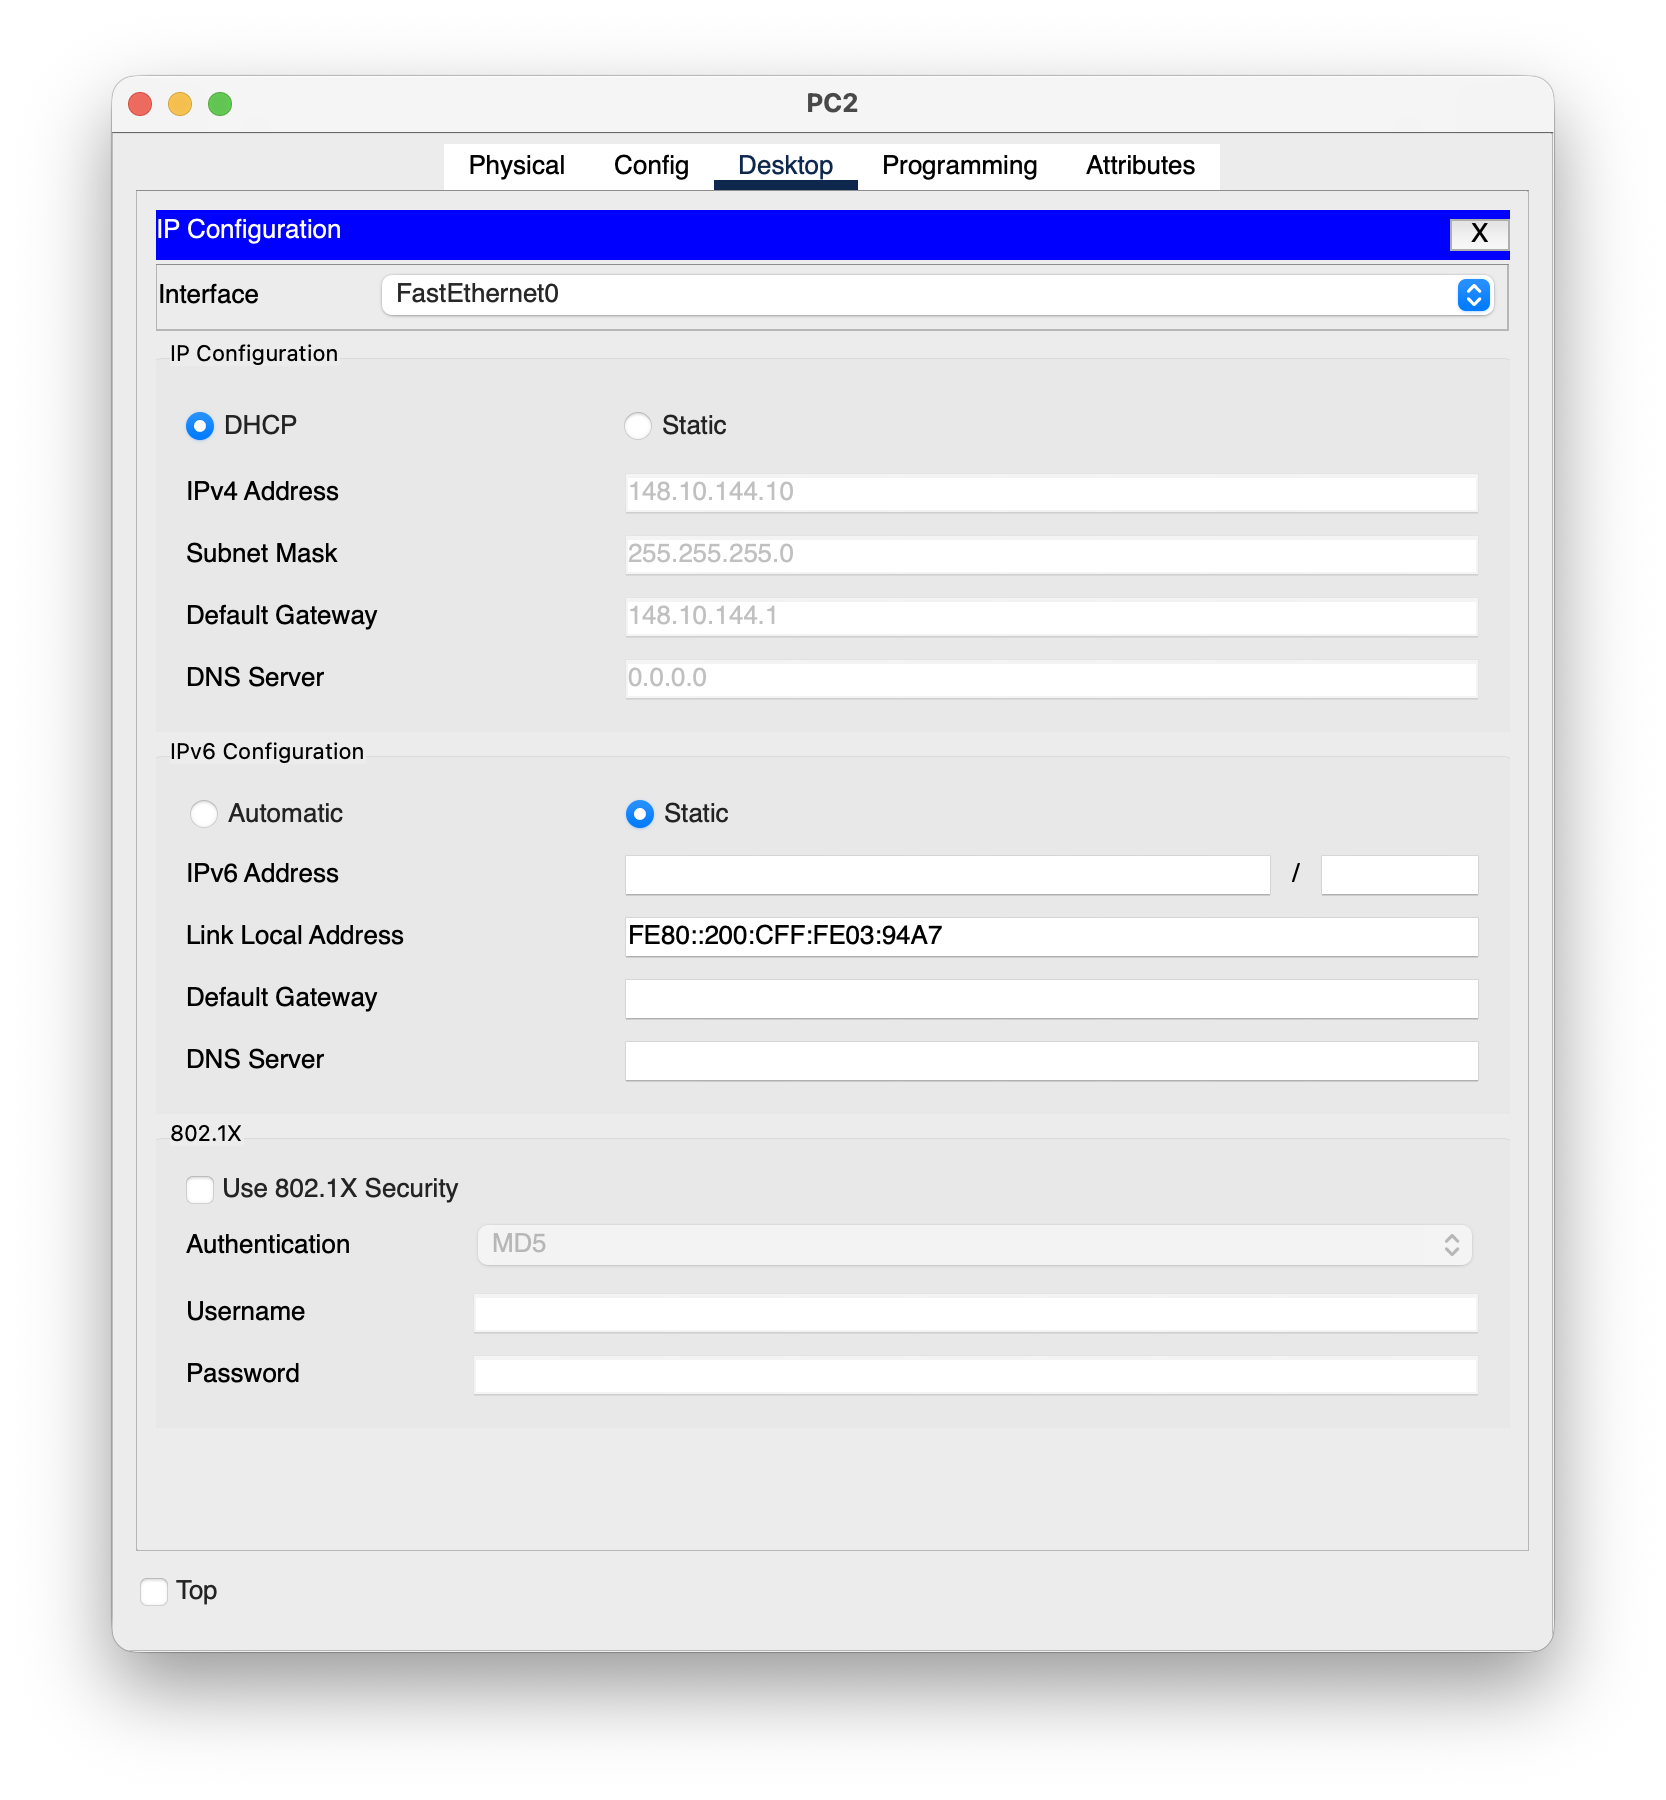
\includegraphics[width=0.85\textwidth]{dhcpMuestra1.png}
\caption{Asignación automática de dirección IP mediante DHCP.}
\label{fig:dhcp1}
\end{figure}

\begin{figure}[H]
\centering
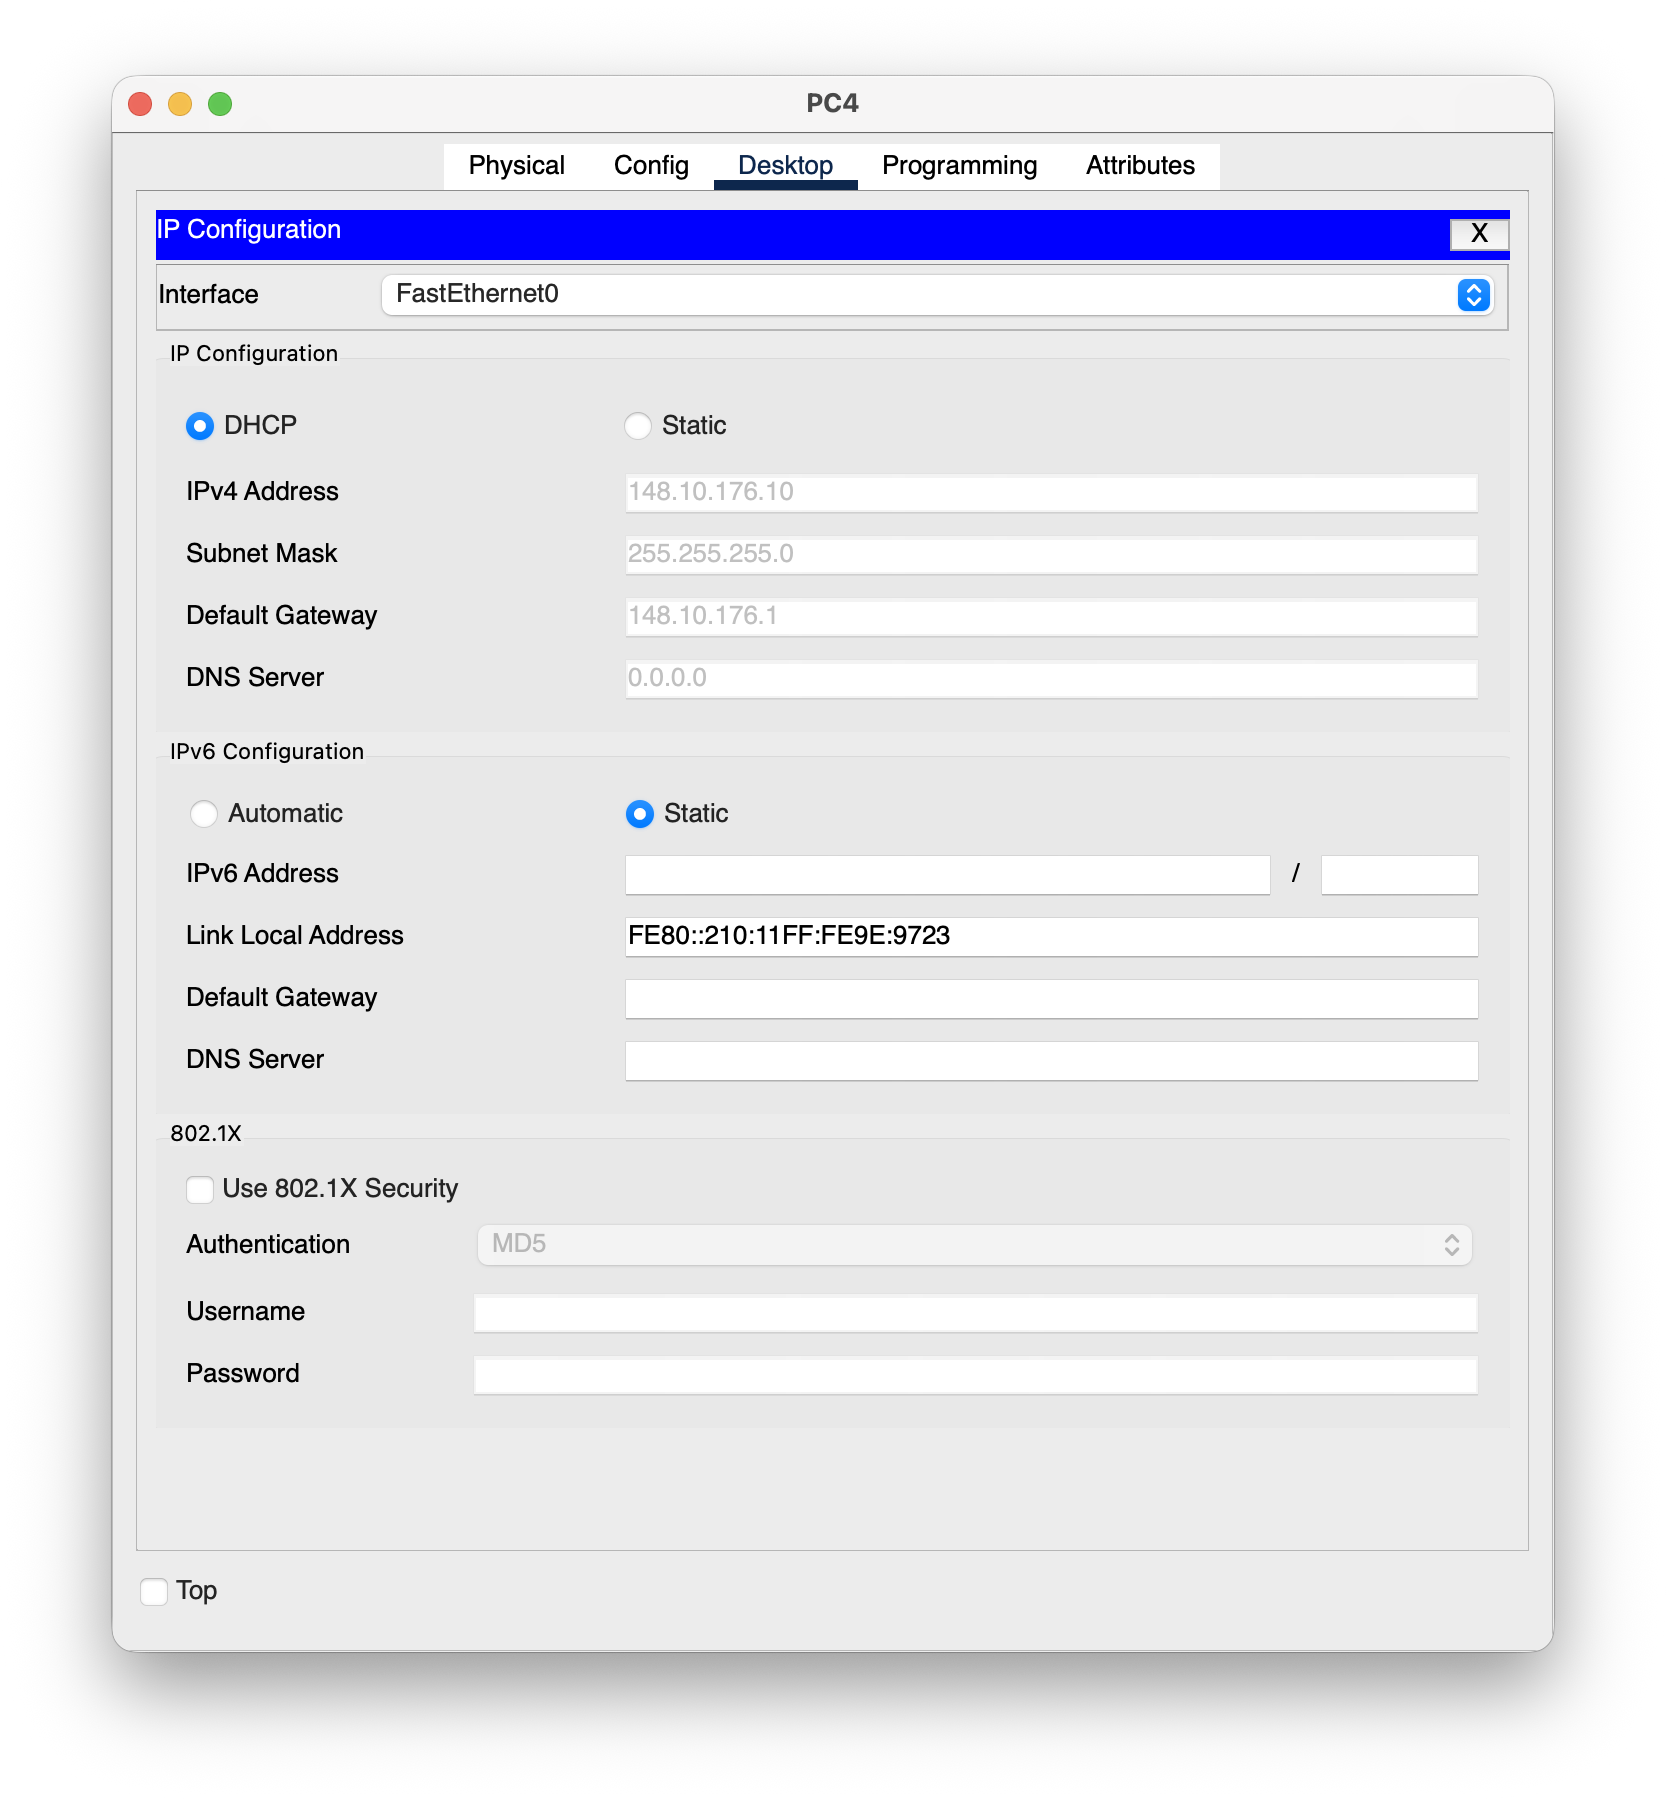
\includegraphics[width=0.85\textwidth]{dhcpMuestra2.png}
\caption{Segunda evidencia de asignación automática mediante DHCP.}
\label{fig:dhcp2}
\end{figure}

La asignación automática permite que los hosts de estas redes reciban una dirección IP perteneciente a la subred correspondiente, así como la máscara de red y la puerta de enlace predeterminada.

\section{Configuración de la salida hacia el ISP}

Uno de los aprendizajes importantes durante la práctica fue distinguir entre el enrutamiento dentro de la red interna y la comunicación con una red externa.

Los routers R1, R2, R3 y R4 intercambian información mediante OSPF. Sin embargo, el ISP no participa en este proceso. Por esta razón, R1 necesita una ruta por defecto que indique que el tráfico destinado a redes desconocidas debe enviarse al ISP.

En R1 se configuró:

\begin{lstlisting}[style=cisco]
ip route 0.0.0.0 0.0.0.0 52.0.0.2
\end{lstlisting}

Posteriormente, esta ruta se anunció mediante OSPF:

\begin{lstlisting}[style=cisco]
router ospf 10
default-information originate
\end{lstlisting}

De esta manera, los demás routers de la red pueden utilizar R1 como salida predeterminada.

\section{Rutas de retorno en el ISP}

Durante las pruebas se observó un comportamiento importante: algunos hosts podían iniciar tráfico hacia el servidor del ISP, pero el ping no se completaba.

El motivo era que el tráfico de ida podía seguir la ruta:

$$
\text{Host} \rightarrow \text{R4/R2} \rightarrow \text{R1} \rightarrow
\text{ISP} \rightarrow \text{Servidor}
$$

pero el servidor necesitaba enviar una respuesta siguiendo el camino inverso:

$$
\text{Servidor} \rightarrow \text{ISP} \rightarrow \text{R1}
\rightarrow \text{R2/R4} \rightarrow \text{Host}
$$

El router ISP no conocía inicialmente las redes internas. Por lo tanto, fue necesario agregar rutas estáticas en ISP utilizando a R1 como siguiente salto.

Las redes internas configuradas fueron:

\begin{lstlisting}[style=cisco]
ip route 148.10.144.0 255.255.255.0 52.0.0.1
ip route 148.10.176.0 255.255.255.0 52.0.0.1
ip route 205.20.3.0 255.255.255.0 52.0.0.1
ip route 206.10.5.0 255.255.255.0 52.0.0.1
\end{lstlisting}

Estas rutas permiten que ISP devuelva correctamente los paquetes hacia las diferentes LAN internas.

\section{Problemas encontrados y solución}

\subsection{Interfaces seriales conectadas incorrectamente}

Uno de los principales problemas durante la configuración fue que los cables seriales no se encontraban conectados a las interfaces que se habían considerado inicialmente.

La configuración original suponía una determinada correspondencia entre interfaces, pero posteriormente se identificó que el enlace R1--R2 utilizaba:

$$
\text{R1 S0/3/0} \leftrightarrow \text{R2 S0/3/1}
$$

mientras que el enlace R2--R3 utilizaba:

$$
\text{R2 S0/3/0} \leftrightarrow \text{R3 S0/3/1}
$$

Esto provocaba que las direcciones IP estuvieran configuradas en interfaces diferentes de aquellas donde realmente se encontraban conectados los cables.

\subsection{Error de solapamiento de redes}

Al intentar configurar R2 se presentó el mensaje:

\begin{verbatim}
% 140.10.0.0 overlaps with Serial0/3/0
\end{verbatim}

Esto ocurrió porque la red \texttt{140.10.0.0/24} todavía estaba configurada en la interfaz antigua de R2.

La solución consistió en eliminar la dirección IP de la interfaz que ya no se utilizaba:

\begin{lstlisting}[style=cisco]
interface s0/3/0
no ip address
shutdown
\end{lstlisting}

Posteriormente se configuró la nueva interfaz con la dirección correspondiente.

Un problema equivalente ocurrió con la red \texttt{140.30.0.0/24}, debido a que R2 todavía conservaba la dirección \texttt{140.30.0.1} en \texttt{S0/2/0}. Se eliminó la configuración de la interfaz anterior antes de reutilizar la red en \texttt{S0/3/0}.

Esto permitió comprender que un router no puede tener dos interfaces activas pertenecientes a la misma subred, ya que las redes quedarían solapadas.

\subsection{Configuración DCE y DTE}

Los enlaces seriales requieren distinguir qué extremo proporciona la señal de reloj. En los enlaces donde R1 o R2 funcionaban como DCE se utilizó:

\begin{lstlisting}[style=cisco]
clock rate 64000
\end{lstlisting}

El extremo DTE no requiere configurar esta velocidad.

Durante la solución de problemas fue necesario verificar la naturaleza de las interfaces debido a que inicialmente los resultados de los comandos de diagnóstico no coincidían con la conexión física que se esperaba.

\subsection{Verificación de las vecindades OSPF}

Al principio, R1 no mostraba vecinos OSPF y tampoco podía hacer ping a R2 a través del enlace correspondiente.

Después de corregir las interfaces y sus direcciones IP, se obtuvo en R2 el mensaje:

\begin{verbatim}
%OSPF-5-ADJCHG: Process 10, Nbr 3.3.3.3
on Serial0/3/0 from LOADING to FULL,
Loading Done
\end{verbatim}

El estado \texttt{FULL} indica que la adyacencia OSPF entre ambos routers se estableció correctamente.

La comprobación de las vecindades mediante:

\begin{lstlisting}[style=cisco]
show ip ospf neighbor
\end{lstlisting}

permitió verificar qué routers estaban intercambiando información mediante OSPF.

\subsection{Rutas de retorno}

Otro problema apareció cuando una PC de una LAN interna intentaba comunicarse con el servidor conectado al ISP.

Por ejemplo:

$$
148.10.176.11 \rightarrow 52.0.1.10
$$

Inicialmente la comunicación fallaba porque, aunque R1 tenía una ruta por defecto hacia ISP, el ISP no tenía una ruta para regresar hacia \texttt{148.10.176.0/24}.

La solución fue agregar en ISP:

\begin{lstlisting}[style=cisco]
ip route 148.10.176.0 255.255.255.0 52.0.0.1
\end{lstlisting}

El mismo principio se aplicó posteriormente a las redes:

\begin{itemize}
\item \texttt{206.10.5.0/24}
\item \texttt{205.20.3.0/24}
\item \texttt{148.10.144.0/24}
\end{itemize}

Esto permitió completar la comunicación bidireccional entre las LAN internas y la red del ISP.

\section{Evidencia de conectividad}

Una vez corregidas las configuraciones de las interfaces, OSPF, DHCP y las rutas de salida y retorno, se realizaron pruebas de conectividad mediante \texttt{ping}.

\begin{figure}[H]
\centering

\includegraphics[width=\textwidth]{pings.png}
\caption{Evidencia de conectividad entre diferentes redes de la topología.}
\label{fig:pings}
\end{figure}

Las pruebas permitieron verificar tanto la conectividad entre los routers como la comunicación entre equipos pertenecientes a diferentes redes.

\section{Aprendizajes}

La práctica permitió reforzar varios conceptos fundamentales de redes.

\subsection{Una interfaz pertenece a una red}

Cada interfaz de un router conecta al dispositivo con una red determinada. Por esta razón, las direcciones IP de las interfaces deben corresponder con las redes que existen físicamente en la topología.

Cambiar un cable de una interfaz a otra no cambia automáticamente la configuración lógica del router. Si se cambia la interfaz física utilizada, también debe revisarse la dirección IP, el estado administrativo, la configuración DCE/DTE y la participación de la interfaz en el protocolo de enrutamiento.

\subsection{OSPF intercambia información de enrutamiento}

OSPF permite que los routers de una misma área intercambien información sobre las redes que conocen. Esto evita tener que crear rutas estáticas individuales entre todos los routers internos.

Una vez establecidas las vecindades, las rutas aprendidas mediante OSPF aparecen en la tabla de enrutamiento identificadas normalmente con la letra \texttt{O}.

\subsection{Una ruta por defecto no sustituye las rutas de retorno}

La existencia de una ruta por defecto en R1 permitió enviar tráfico hacia el ISP cuando no existía una ruta más específica.

Sin embargo, esto no significa que el ISP conozca automáticamente las redes internas. Para completar una comunicación IP se necesita un camino de ida y un camino de regreso.

Este fue uno de los aprendizajes más importantes de la práctica:

\begin{quote}
Una comunicación exitosa requiere que exista una ruta válida tanto para llegar al destino como para regresar al origen.
\end{quote}

\subsection{DHCP simplifica la configuración de los hosts}

Al configurar R4 como servidor DHCP, los equipos conectados a S3 y S4 pudieron obtener automáticamente sus parámetros de red.

Esto reduce la necesidad de configurar manualmente cada host y disminuye el riesgo de errores de direccionamiento.

\subsection{Uso de comandos de diagnóstico}

Durante la solución de problemas se utilizaron comandos como:

\begin{lstlisting}[style=cisco]
show ip interface brief
show ip protocols
show ip ospf neighbor
show ip route
ping
\end{lstlisting}

Estos comandos permiten analizar diferentes capas del funcionamiento de la red:

\begin{itemize}
\item \texttt{show ip interface brief}: estado y direccionamiento de las interfaces.
\item \texttt{show ip protocols}: protocolos de enrutamiento configurados y redes anunciadas.
\item \texttt{show ip ospf neighbor}: vecindades OSPF establecidas.
\item \texttt{show ip route}: rutas conocidas por el router.
\item \texttt{ping}: comprobación de conectividad entre dos direcciones IP.
\end{itemize}

El orden de utilización de estas herramientas también resulta importante. Ante un problema de conectividad, es conveniente comprobar primero las interfaces y los enlaces directos, posteriormente las vecindades de routing, después las tablas de rutas y finalmente la conectividad extremo a extremo.

\section{Conclusiones}

La práctica permitió implementar una red con múltiples routers utilizando OSPF como protocolo de enrutamiento dinámico y DHCP para la configuración automática de determinados hosts.

Además de la configuración inicial, los problemas encontrados permitieron comprender que una topología de red debe analizarse tanto desde su estructura física como desde su configuración lógica. La modificación de una interfaz utilizada por un enlace serial puede provocar conflictos de direccionamiento si las configuraciones anteriores no son eliminadas.

También se comprobó la importancia de las rutas de retorno. La configuración de una ruta por defecto en R1 permitió enviar tráfico hacia el ISP, pero fue necesario agregar rutas estáticas en ISP para que las respuestas pudieran regresar hacia las LAN internas.

Finalmente, la utilización conjunta de \texttt{show ip interface brief}, \texttt{show ip ospf neighbor}, \texttt{show ip protocols}, \texttt{show ip route} y \texttt{ping} permitió identificar y solucionar los problemas de conectividad de manera sistemática.

La práctica reforzó así la relación entre direccionamiento IPv4, interfaces de routers, enlaces seriales, OSPF, rutas por defecto, rutas estáticas, DHCP y conectividad extremo a extremo.

\end{document}
